
\subsection{Account List Display}
\label{sec:account}

The Account List screen displays the name and the current amount of the accounts that the user has added. It also displays a flag indicating  whether or not an account has been marked as default. It allows the user to delete an account, or set it as default by swiping the list item left. When an account item is tapped, the user is taken to a screen where the account details can be viewed and edited. Note that an account marked as default cannot be deleted, so when swiping left, the only available option is \"Edit\", which has the same functionality as tapping the account list item.

\subsubsection{Application Screenshots}
\label{sec:account-screenshots}

\begin{figure}[h]
\begin{subfigure}{0.5\textwidth}
  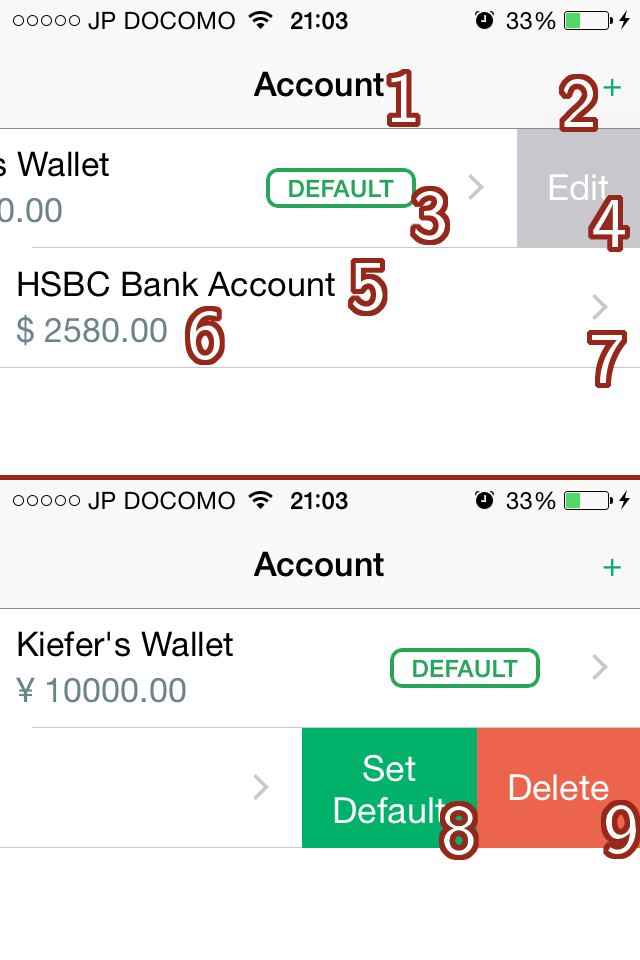
\includegraphics[scale=0.35]{ACC-0002-1} 
  \caption{Account List Screen}
  \label{fig:account-1}
\end{subfigure}
\begin{subfigure}{0.5\textwidth}
  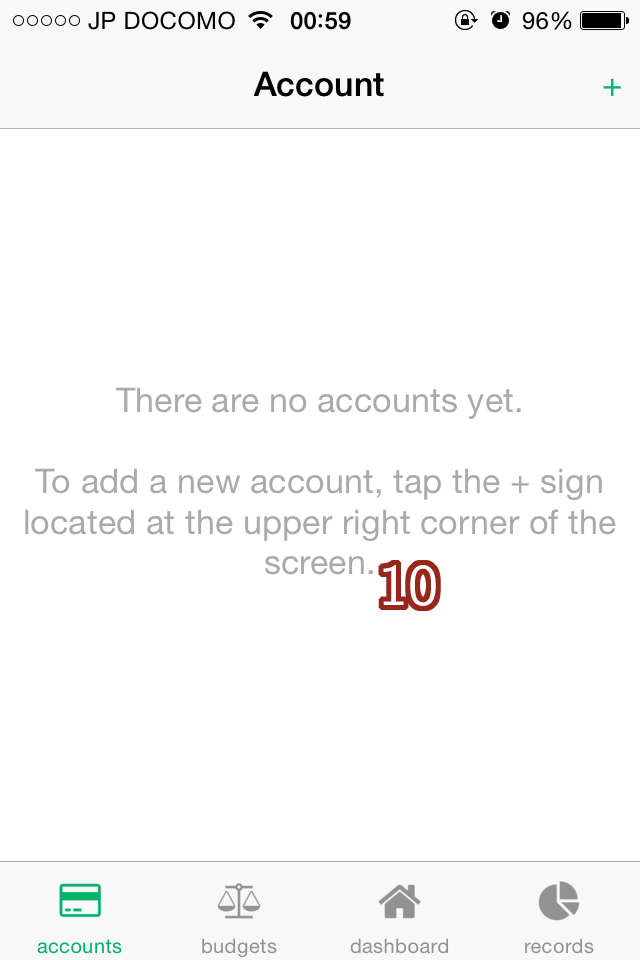
\includegraphics[scale=0.35]{ACC-0002-2}
  \caption{Empty Account List}
  \label{fig:account-2}
\end{subfigure}
\caption{Account List Screenshots}
\label{Account List Screenshots}
\end{figure}

\screentable{
	\header{Screen Component}
    	{Type}
        {Description}
    \row{1. Screen Title}
    	{Label Title}
        {Localization Key: MENULABEL\_ACCOUNT}
    \row{2. Add Button}
    	{Button}
        {When tapped, the screen transitions to the Add Account Screen. (See section: \nameref{sec:add-account})} 
    \row{3. Default Icon}
    	{View Element}
        {An indicator showing whether or not an account is marked as default. There can only be one default account at any one time. \doublenewline
        
        Localization Key: LABEL\_DEFAULT}
    \row{4. Edit Button}
    	{Table Cell Button}
        {This button is displayed when the swiped cell is not a default account. When tapped, the screen transitions to the Edit Account Screen (See section: \nameref{sec:edit-account}) \doublenewline
        
        Localization Key: BUTTON\_EDIT}
       \row{5. Account Name Label}
    	{Label}
        {A label that displays the name of the account.} 
    \row{6. Amount Label}
    	{Label}
        {A label that displays the account's currency and the amount.} 
    \row{7. Chevron Icon}
    	{Table cell icon}
        {Indicates that when the entire cell can be tapped. When tapped, the screen transitions to the Edit Account Screen (See section: \nameref{sec:edit-account})}
}


\screentable{
	\header{Screen Component}
    	{Type}
        {Description}
    \row{8. Set Default Button}
    	{Table Cell Button}
        {This button is displayed when the swiped cell is as default account. \doublenewline
        When tapped, the cell will slide back and will be marked as default. The previously default cell will slide too, indicating that it was updated and unmarked. \doublenewline
        
        Localization Key: BUTTON\_SET\_DEFAULT}
    \row{9. Delete Button}
    	{Table Cell Button}
        {When tapped, the account is deleted and the cell slides away to disappear. \doublenewline
        Localization Key: BUTTON\_DELETE}
    \row{10. No Accounts Guide}
    	{Label}
        {This label is displayed when there are no accounts present. \doublenewline 
        
        This scenario theoretically should not happen under normal circumstances, as there is no way for the user to delete an account marked as default, and when the app is freshly installed, there will be one account available, and it is marked as default. \doublenewline
        
        Localization Key: GUIDELABEL\_NO\_ACCOUNTS} 
}